% !TEX program = xelatex
% Статья: Исследование эффективности использования зеркально-усиленной
% лидарной системы для нейросетевой сегментации и классификации объектов.
% Оформление — шаблон НИТУ «МИСиС» (misisarticle.cls), XeLaTeX.
% Текст перенесён из репозитория статьи ГрафиКон-2026 (шаблон ceurart).

\documentclass{misisarticle}

% --- Дополнительные пакеты для перенесённого текста ---
\usepackage{listings}
\lstset{breaklines=true}
\renewcommand{\lstlistingname}{Листинг}
\usepackage{subcaption}
\renewcommand{\thesubfigure}{\asbuk{subfigure}}
\captionsetup[subfigure]{labelformat=parens}

% Для векторной графики (блок-схема конвейера)
\usepackage{tikz}
\usetikzlibrary{arrows.meta,positioning}

% Моноширинный шрифт с кириллицей для листинга псевдокода
\IfFontExistsTF{DejaVu Sans Mono}{%
  \newfontfamily\monocyr{DejaVu Sans Mono}[Scale=MatchLowercase]%
}{%
  \let\monocyr\ttfamily
}

% --- Классификационные коды ---
\grnti{47.01.07, 47.01.09}
\asjc{1707, 2207}
\oecd{1020, 1070}

% --- Название ---
\title{Исследование эффективности использования зеркально-усиленной
лидарной системы для нейросетевой сегментации и классификации объектов}

% --- Авторы: \misisauthor{ФИО}{аффилиация}{город, страна}{email} ---
\misisauthor{П.~С.~Федулов}{кафедра инженерной кибернетики НИТУ «МИСиС»}{Москва, Россия}{m2308242@edu.misis.ru}
\misisauthor{В.~В.~Силаев}{кафедра инженерной кибернетики НИТУ «МИСиС»}{Москва, Россия}{vs.silaev@yandex.ru}

% --- Аннотация и ключевые слова ---
\abstract{%
  Зеркальное усиление — простой способ повысить плотность и полноту
  облаков точек механических лидаров без замены сенсора, однако оно
  требует точной калибровки положения зеркала относительно лидара, а
  интерпретация полученных данных облегчается при наличии цвета.
  Работа посвящена двум взаимосвязанным задачам для
  зеркально-усиленной лидарной системы на базе Velodyne VLP-16 и
  USB-камеры $640 \times 480$. Во-первых, предложен метод автоматической
  калибровки плоскости зеркала по данным самого лидара: облако
  разделяется на прямую и отражённую части, а параметры зеркала
  итеративно уточняются алгоритмом ICP в контуре обратной связи
  реального времени, без специальных мишеней; на серии из семи запусков
  из различных начальных рассогласований контур устойчиво сходится, а
  итоговые параметры зеркала ($\psi = 32{,}1^{\circ}$, $c_y = 5{,}2$~мм)
  обеспечивают слияние прямого и отражённого облаков без видимого
  расслоения. Во-вторых, описан
  конвейер цветовой регистрации объединённого (прямого и отражённого)
  облака точек по изображению камеры с интерактивной калибровкой
  внешних параметров камера--лидар; на записи длительностью $78$~с
  достигается покрытие $\sim 24\%$ точек с приростом $\sim 33\%$ от
  зеркального канала. Реализация оформлена в виде двух пакетов ROS~2
  (C++/PCL и Python/OpenCV) и апробирована на реальной установке.
}

\keywords{%
  LiDAR, зеркальное усиление, калибровка зеркала, ICP, Velodyne VLP-16,
  цветовая регистрация облака точек, калибровка камера-лидар
}

\begin{document}

\maketitle

% ============================================================
\section{Введение}

Механические лидары среднего ценового сегмента, к которым относится и
используемый в настоящей работе Velodyne VLP-16, формируют облака точек
с ограниченным числом сканирующих каналов (у VLP-16 их 16) и,
как следствие, с низкой плотностью измерений, особенно по вертикали и
на дальних дистанциях. Это затрудняет решение прикладных задач —
картографирования, навигации, распознавания объектов, — где требуются
плотные и полные трёхмерные данные~\cite{khoshelham2018benchmark}.

В работе~\cite{VisFed26} был предложен метод зеркального
усиления механических лидарных систем: плоское зеркало, установленное в
поле зрения сенсора, отражает часть лазерных лучей и формирует
дополнительный (зеркальный) канал сканирования, что позволяет повысить
плотность и полноту облака без замены аппаратуры. Схожие идеи
использования зеркал для расширения зоны измерения лидара
рассматривались и в других
работах~\cite{Matsubara2020MirrorLiDAR,Pogacnik2022MultiperspectiveLiDAR}.
При этом работоспособность метода критически зависит от точности, с
которой известно положение зеркала относительно лидара: даже небольшое
рассогласование в ориентации плоскости зеркала приводит к заметному
смещению отражённого облака и, как следствие, к ошибкам в объединённых
данных. В упомянутых работах калибровка зеркала выполнялась либо
вручную, либо по калибровочным мишеням~\cite{Kibii2022MirrorCalibration},
что требует дополнительного оборудования и времени и не позволяет
отслеживать дрейф параметров в процессе эксплуатации.

Отдельной практической задачей является интерпретация полученных
облаков: бесцветные геометрические данные сложны для визуального
анализа и для задач, использующих текстурную информацию. В системах
лидарно-инерциальной и совмещённой лидарно-визуальной одометрии и
картографирования, таких как FAST-LIO2~\cite{fastlio2} и
R3LIVE~\cite{r3live}, построение цветных облаков точек является
неотъемлемой частью конвейера. Перенос этой идеи на зеркально-усиленную
систему требует согласованной калибровки трёх элементов: лидара,
зеркала и камеры.

Настоящая работа продолжает линию исследований~\cite{VisFed26}
и посвящена двум взаимосвязанным задачам, возникающим при практической
реализации зеркально-усиленной лидарной системы. Вклад работы состоит
в следующем:
\begin{enumerate}
  \item предложен метод автоматической калибровки положения плоского
        зеркала относительно лидара по данным самого сенсора: облако
        точек разделяется на прямую и отражённую части, а параметры
        зеркала итеративно уточняются алгоритмом ICP~\cite{Besl1992ICP}
        в контуре обратной связи реального времени, без калибровочных
        мишеней;
  \item описан конвейер цветовой регистрации объединённого (прямого и
        отражённого) облака точек по изображению камеры, включающий
        интерактивную калибровку внешних параметров камера--лидар;
  \item оба метода реализованы в виде пакетов ROS~2 и апробированы на
        реальной экспериментальной установке (Velodyne VLP-16,
        плоское зеркало, USB-камера); предложена воксельная метрика
        прироста плотности облака за счёт зеркального канала.
\end{enumerate}

Далее статья организована следующим образом. В разделе~2 формулируется
задача и вводятся обозначения. Раздел~3 содержит описание методов:
модели зеркального канала, алгоритма ICP-калибровки с обратной связью и
конвейера цветовой регистрации. В разделе~4 описаны экспериментальная
установка и результаты. Раздел~5 посвящён обсуждению результатов и
ограничений подхода. В заключении сформулированы выводы и направления
дальнейшей работы.

% ============================================================
\section{Постановка задачи}

Рассматривается стационарная измерительная система, состоящая из
механического лидара $L$, плоского зеркала $M$ и цифровой камеры $C$,
жёстко закреплённых на общем основании. Все точки рассматриваются в
системе координат лидара; положение начала системы координат совпадает
с оптическим центром лидара.

Плоскость зеркала задаётся центром
$c = (c_x, c_y, c_z)^{\top} \in \mathbb{R}^3$ и единичной нормалью
$n \in \mathbb{R}^3$, $\|n\| = 1$. В настоящей работе принимается
допущение о вертикальной установке зеркала: его нормаль лежит в
горизонтальной плоскости и параметризуется одним углом $\psi$ (yaw):
\begin{equation}
  n(\psi) = (\cos\psi,\; \sin\psi,\; 0)^{\top}.
  \label{eq:normal}
\end{equation}
Габариты зеркала задаются шириной $w$ и высотой $h$.

Каждое облако точек $P$, формируемое лидаром, естественным образом
распадается на две части. Прямая часть $P_n$ содержит точки, измеренные
лучами, не испытавшими отражения. Зеркальная часть $P_m$ содержит точки,
измеренные лучами, отражёнными от зеркала: такие точки лежат за
плоскостью зеркала, то есть $(p - c)^{\top} n > 0$, и внутри фрустума,
образованного началом координат и контуром зеркала. Отражением точки
$p \in P_m$ в плоскости зеркала называется точка
\begin{equation}
  p^{*} = p - 2\,\bigl((p - c)^{\top} n\bigr)\, n,
  \label{eq:reflect}
\end{equation}
соответствующая положению, которое имел бы измеренный объект, если бы
луч прошёл напрямую (эквивалентно — измерение, выполненное
<<виртуальным лидаром>>, зеркально симметричным $L$ относительно
плоскости $M$).

При точно известных параметрах $(c, \psi)$ отражённое облако
$P_m^{*} = \{\, p^{*} \mid p \in P_m \,\}$ должно быть геометрически
согласовано с прямым облаком $P_n$: одни и те же объекты сцены,
видимые в обоих каналах, должны совпадать. На практике параметры
зеркала известны лишь приближённо (после механической установки), что
приводит к систематическому смещению $P_m^{*}$ относительно $P_n$.

Сформулируем две задачи, решаемые в работе.

\textbf{Задача 1 (калибровка зеркала).} По последовательности облаков точек
$P^{(k)}$ одной и той же статичной сцены оценить параметры
$(c, \psi)$ плоскости зеркала так, чтобы минимизировать рассогласование
между отражённым облаком $P_m^{*}(c, \psi)$ и прямым облаком $P_n$.
Калибровка $(c, \psi)$ должна выполняться автоматически, по данным самого лидара,
без специальных мишеней, и сопровождаться численным критерием сходимости.
Ширина зеркала $w$ при этом фиксируется на заведомо большом значении, а после сходимости
контура уточняется вручную по видимому совпадению границ фрустума с краями зеркальной поверхности.

\textbf{Задача 2 (цветовая регистрация).} По изображению камеры $C$ и
объединённому облаку $P_n \cup P_m^{*}$ присвоить каждой точке облака
цвет соответствующего пикселя изображения. Для этого требуется оценить
внешние параметры камеры относительно лидара --- матрицу
$T_{lc} = [\,R_{lc} \mid t_{lc}\,]$ --- и обеспечить корректную
проекцию точек на изображение с учётом внутренних параметров и
дисторсии камеры.

Обе задачи рассматриваются для статичной сцены и жёсткой механической
связи элементов системы; вопросы динамики и взаимных окклюзий в
настоящей работе не рассматриваются (см. раздел~5).

% ============================================================
\section{Методы и алгоритмы}

\subsection{Модель зеркального канала}
\label{sec:mirror-model}

Зеркальный канал описывается моделью плоского зеркала
с параметрами $(c, \psi, w, h)$, введёнными в разделе~2. Обработка
каждого входного облака $P$ начинается с разделения его точек на
прямые и зеркальные. Точка $p$ относится к зеркальной части $P_m$,
если выполнены два условия. Первое --- точка лежит за плоскостью
зеркала:
\begin{equation}
  (p - c)^{\top} n(\psi) > 0,
  \label{eq:behind}
\end{equation}
где нормаль $n(\psi)$ определена в~\eqref{eq:normal}. Второе --- точка
находится внутри фрустума зеркала, то есть внутри угловой области,
натянутой из начала координат на контур зеркала. Пусть
\begin{equation}
  t(\psi) = (-\sin\psi,\; \cos\psi,\; 0)^{\top}
\end{equation}
--- единичный касательный вектор к плоскости зеркала в горизонтальной
плоскости, а $u = (0,0,1)^{\top}$ --- вертикальное направление. Тогда
граничные точки зеркала по ширине задаются как
$M_L = c - \frac{w}{2}\,t$ и $M_R = c + \frac{w}{2}\,t$, а нормали
граничных плоскостей фрустума --- как
\begin{equation}
  n_L = \frac{u \times M_L}{\|u \times M_L\|}, \qquad
  n_R = \frac{M_R \times u}{\|M_R \times u\|},
\end{equation}
при этом условие попадания точки внутрь фрустума по горизонтали имеет
вид $n_L^{\top} p \ge 0$ и $n_R^{\top} p \ge 0$. Аналогичные проверки
выполняются по вертикали с использованием высоты $h$ зеркала.
В описываемой конфигурации эксперимента зеркало перекрывает всё
вертикальное поле обзора лидара, поэтому вертикальная проверка фрустума
не ограничивает разбиение: все точки, прошедшие условие \eqref{eq:behind}
и горизонтальную проверку, относятся к зеркальной части независимо от $h$.
Высота $h$ зафиксирована в модели, но не влияет на результат.
Совокупность условий \eqref{eq:behind} и проверок фрустума определяет
разбиение $P = P_n \cup P_m$.

Каждая зеркальная точка затем отражается в плоскости зеркала по
формуле~\eqref{eq:reflect}, что соответствует преобразованию
Хаусхолдера относительно плоскости $(c, n)$. Результатом является
отражённое облако $P_m^{*}$, которое при корректных параметрах зеркала
должно быть геометрически согласовано с прямым облаком $P_n$.
Объединённое облако $P_n \cup P_m^{*}$ публикуется в топик
\texttt{/aligned\_cloud} и используется как для калибровки
(п.~\ref{sec:icp-calib}), так и для цветовой регистрации
(п.~\ref{sec:color}).

Геометрия зеркального канала (прямой и отражённый лучи, виртуальный
лидар, фрустум) показана на рис.~\ref{fig:geometry}.

\begin{figure}[t]
  \centering
  \begin{minipage}{0.85\linewidth}
    \centering
    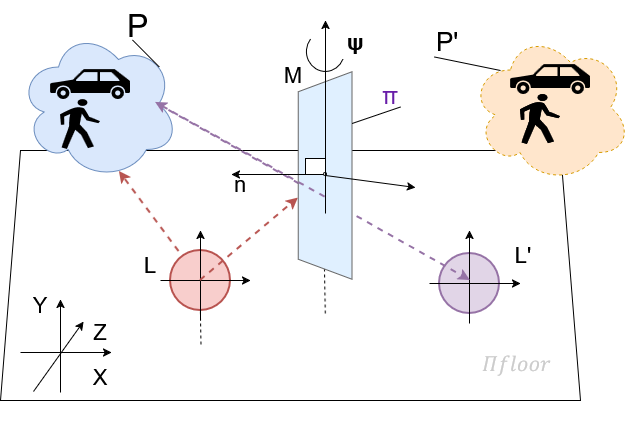
\includegraphics[width=\linewidth]{figures/mirror.png}
  \end{minipage}
  \caption{Схема формирования виртуального канала: прямое облако точек $P$,
    зеркальное облако точек $P'$, лидар $L$ и виртуальный лидар $L'$,
    $n$ – нормаль к плоскости $\pi$ зеркала $M$, ориентированная углом $\psi$,
    опорная плоскость в глобальных координатах ($X$, $Y$, $Z$) --- $\pi_{\mathrm{floor}}$}
  \label{fig:geometry}
\end{figure}

\subsection{ICP-калибровка положения зеркала с обратной связью}
\label{sec:icp-calib}

Идея метода состоит в том, чтобы трактовать рассогласование между
$P_m^{*}$ и $P_n$ как функцию ошибки в параметрах зеркала и устранять
его итеративно. Небольшая ошибка в ориентации $\psi$ и положении $c$
плоскости зеркала приводит к жёсткому (в первом приближении) смещению и
повороту всего отражённого облака $P_m^{*}$ относительно прямого
облака $P_n$. Следовательно, оценив это смещение алгоритмом ICP, можно
вычислить поправку к параметрам зеркала.

\textbf{Выравнивание ICP.} Для снижения вычислительной нагрузки оба
облака предварительно прореживаются воксельным фильтром с размером
листа $0{,}1$~м. Пусть $S = \{s_i\}$ --- прореженное отражённое облако
$P_m^{*}$, а $Q$ --- прореженное прямое облако $P_n$. Алгоритм
ICP~\cite{Besl1992ICP} в point-to-point постановке (реализация
библиотеки PCL~\cite{Rusu2011PCL}) находит жёсткое преобразование
\begin{equation}
  T^{*} = \arg\min_{T \in SE(3)} \sum_{i} \bigl\| T\, s_i - q(i) \bigr\|^2,
  \label{eq:icp}
\end{equation}
где $q(i) \in Q$ --- ближайшая к $T s_i$ точка прямого облака;
соответствия с расстоянием больше $0{,}2$~м отбрасываются. Число
итераций ограничено 30, что обеспечивает работу в темпе поступления
кадров лидара.

\textbf{Обновление параметров зеркала.} Из найденного преобразования
$T^{*}$ извлекаются поправки $(\Delta x, \Delta y, \Delta\psi)$:
поступательные составляющие вдоль горизонтальных осей и угловая
составляющая вокруг вертикальной оси. Параметры зеркала обновляются с
коэффициентами усиления:
\begin{equation}
  c \leftarrow c + \bigl(g_x \Delta x,\; g_y \Delta y,\; 0\bigr)^{\top},
  \qquad
  \psi \leftarrow \psi + g_{\psi}\, \Delta\psi,
  \label{eq:update}
\end{equation}
где в используемой конфигурации $g_x = 0$, $g_y = g_{\psi} = 0{,}5$.
Значение $0{,}5$ соответствует геометрии отражения: малая ошибка в
положении или ориентации зеркала порождает удвоенное смещение или
поворот отражённого облака, поэтому к параметрам применяется половина
оценённой ICP поправки; это же подавляет осцилляции контура.
Отражение~\eqref{eq:reflect} зависит от центра зеркала только через
проекцию $c^{\top} n$, поэтому независимо наблюдаема лишь одна
поступательная степень свободы плоскости; калибруется $c_y$, а $c_x$
фиксируется ручной инициализацией ($g_x = 0$).

\textbf{Критерий остановки.} Контур работает в потоковом режиме:
поправки применяются к каждому вновь поступающему кадру. Обновление
пропускается, когда норма поправки становится меньше порога
$10^{-3}$, либо когда среднеквадратичная ошибка совмещения
\begin{equation}
  E = \sqrt{\frac{1}{|S|}
    \sum_{s_i \in S} \bigl\| T^{*} s_i - q(i) \bigr\|^2}
  \label{eq:rmse}
\end{equation}
опускается ниже заданного порога $\varepsilon$ (значение подбирается
под масштаб $E$ для конкретной сцены; использованное в экспериментах
значение указано в разделе~4) и ICP на кадре сошёлся. В отличие от внутренней
метрики ICP, при вычислении $E$ отсечка соответствий по расстоянию не
применяется: суммирование ведётся по всем точкам прореженного
отражённого облака. Поскольку прямое и отражённое облака покрывают
существенно различные участки сцены, абсолютное значение $E$
определяется главным образом геометрией сцены, а не остаточной
ошибкой калибровки; поэтому $E$ служит относительным критерием
останова, а не мерой точности. После остановки контура оценённые
параметры фиксируются и используются для отражения облаков без
дальнейшей коррекции.

Псевдокод полного цикла обработки одного кадра приведён в
листинге~\ref{lst:feedback}.

\begin{lstlisting}[
  basicstyle=\scriptsize\monocyr,
  frame=single,
  caption={Псевдокод калибровки зеркала с обратной связью (один кадр).},
  label={lst:feedback}
]
вход: облако P, параметры (c, psi, w, h)
P_n, P_m <- разделить P по (3) и фрустуму
P_m* <- отразить P_m по (2)     # безусловно
если контур активен:
  S, Q <- воксельный фильтр P_m*, P_n (0.1 м)
  T* <- ICP(S -> Q)             # (6), 0.2 м, 30 итер.
  (dx, dy, dpsi) <- поправки из T*
  если |dx|,|dy|,|dpsi| >= delta:
    c <- c + (0, g_y*dy, 0)     # (7)
    psi <- psi + g_psi*dpsi
  если E < eps и автовыключение:
    стоп, зафиксировать (c, psi)
выход: P_n U P_m* -> /aligned_cloud
\end{lstlisting}

Помимо собственно калибровки, реализация вычисляет вспомогательную
метрику плотности облака: сцена разбивается на воксели, и для прямого и
объединённого облаков оценивается среднее число точек на единицу
объёма (точек/м\textsuperscript{3}). Отношение этих величин даёт
количественную характеристику зеркального усиления (иллюстративное
применение --- в разделе~4; подробное исследование метрики выполнено
в~\cite{VisFed26}).

\textbf{Калибровка ширины зеркала.} Описанный выше контур оценивает
положение $c$ и ориентацию $\psi$ плоскости зеркала, но не его ширину
$w$. На этапе работы контура $w$ устанавливается заведомо большой
(«бесконечное зеркало»), чтобы фрустум не отбрасывал потенциальные
зеркальные точки. После сходимости контура $w$ уточняется вручную:
последовательно перебираются значения $w$, визуально контролируя
в RViz совпадение боковых граней фрустума с краями зеркальной
поверхности. При $w < w_{\text{ист}}$ часть зеркальных точек
отбрасывается; при $w > w_{\text{ист}}$ в зеркальную часть попадают
точки сцены, не являющиеся отражениями. Правильное значение $w$
минимизирует обе ошибки. Высота $h$ в рассматриваемой конфигурации не
калибруется, поскольку зеркало перекрывает всё вертикальное поле
обзора лидара.

\subsection{Цветовая регистрация облака точек}
\label{sec:color}

Цветовая регистрация выполняется проекцией точек объединённого облака
на изображение камеры. Камера описывается стандартной моделью
камеры-обскуры с матрицей внутренних параметров
\begin{equation}
  K = \begin{pmatrix}
    f_x & 0   & c_x \\
    0   & f_y & c_y \\
    0   & 0   & 1
  \end{pmatrix}
\end{equation}
и вектором коэффициентов дисторсии Брауна
$D = (k_1, k_2, p_1, p_2, k_3)$; проекция с учётом дисторсии
выполняется функцией \texttt{cv2.projectPoints} библиотеки OpenCV.
Внутренние параметры камеры предварительно откалиброваны по
шахматной мишени методом Жанга~\cite{Zhang2000Calibration}.

Переход из системы координат лидара в систему координат камеры
задаётся внешними параметрами $T_{lc} = [\,R_{lc} \mid t_{lc}\,]$,
$p_C = R_{lc}\, p_L + t_{lc}$. С учётом взаимной ориентации сенсоров
на установке матрица поворота параметризуется одним углом $\varphi$
(yaw):
\begin{equation}
  R_{lc} = R_b\, R_z(\varphi), \qquad
  R_b = \begin{pmatrix}
    0 & -1 & 0 \\
    0 & 0 & -1 \\
    1 & 0 & 0
  \end{pmatrix},
  \label{eq:rlc}
\end{equation}
где $R_b$ --- фиксированный базовый поворот, согласующий оси сенсоров
(оптическая ось камеры параллельна продольной оси лидара), а
$R_z(\varphi)$ --- поворот вокруг вертикальной оси. Таким образом,
внешняя калибровка сводится к подбору четырёх параметров:
$(t_x, t_y, t_z, \varphi)$. Для жёстко смонтированной установки этого
достаточно: оставшиеся две угловые степени свободы устранены
конструкцией крепления, а их малые остаточные ошибки поглощаются
подбором $\varphi$ и $t_{lc}$.

Подбор параметров выполняется интерактивно: кадр лидарного потока и
изображение камеры фиксируются, после чего оператор с помощью
ползунков графического интерфейса изменяет $(t_x, t_y, t_z, \varphi)$
до визуального совпадения проецируемого облака с объектами на
изображении. Найденные значения сохраняются в конфигурацию и далее
используются в потоковом режиме.

При покраске каждая точка $p$ объединённого облака переводится в
систему камеры, проецируется на изображение и, если выполнены условия
$z_C > 0{,}1$~м (точка перед камерой) и попадания проекции в границы
кадра, получает цвет соответствующего пикселя. Процедура едина для
прямых и отражённых точек, поскольку последние уже приведены отражением
\eqref{eq:reflect} в систему координат лидара. Результат публикуется
в топик \texttt{/colored\_cloud}.

Следует отметить, что взаимные окклюзии (точка облака соответствует
объекту, не видимому камерой) в текущей реализации не обрабатываются:
такие точки получают цвет фонового объекта. Это ограничение обсуждается
в разделе~5.

Полный конвейер обработки данных показан на рис.~\ref{fig:pipeline}.

\begin{figure}[t]
  \centering
  \resizebox{0.98\linewidth}{!}{%
  \begin{tikzpicture}[
      font=\footnotesize,
      block/.style={draw, rounded corners=2pt, align=center,
                    minimum height=8mm, inner sep=3pt},
      topic/.style={align=center, font=\footnotesize\ttfamily},
      arr/.style={-{Stealth[length=2mm]}, thick}
    ]
    \node[topic] (in) {/velodyne\_points};
    \node[block, right=3mm of in] (split) {разделение\\(плоскость, фрустум)};
    \node[block, right=3mm of split] (refl) {отражение\\по~\eqref{eq:reflect}};
    \node[block, right=3mm of refl] (icp) {ICP-контур\\обновление $c_y$, $\psi$};
    \node[block, right=3mm of icp] (merge) {объединение};
    \node[topic, right=3mm of merge] (aligned) {/aligned\_cloud};
    \node[block, below=9mm of aligned] (color) {покраска\\по $K$, $T_{lc}$};
    \node[topic, left=3mm of color] (cam) {/camera/image};
    \node[topic, right=3mm of color] (out) {/colored\_cloud};
    \draw[arr] (in) -- (split);
    \draw[arr] (split) -- (refl);
    \draw[arr] (refl) -- (icp);
    \draw[arr] (icp) -- (merge);
    \draw[arr] (merge) -- (aligned);
    \draw[arr] (aligned) -- (color);
    \draw[arr] (cam) -- (color);
    \draw[arr] (color) -- (out);
    \draw[arr, dashed] (icp.north) to[out=55, in=125]
      node[midway, above, font=\footnotesize] {$(c_y, \psi)$} (refl.north);
  \end{tikzpicture}}
  \caption{Блок-схема конвейера обработки данных: блоки от разделения
    до объединения выполняются пакетом ROS~2 \texttt{icp\_registration}
    (C++/PCL), покраска --- пакетом \texttt{colorize\_live\_pkg}
    (Python/OpenCV); пунктиром показана обратная связь по параметрам
    зеркала.}
  \label{fig:pipeline}
\end{figure}

% ============================================================
\section{Результаты экспериментов}

\subsection{Экспериментальная установка}

Эксперименты проведены на стационарной установке (рис.~\ref{fig:setup}),
включающей механический лидар Velodyne VLP-16 (16 сканирующих каналов,
заявленная точность дальнометрии $\pm 3$~см~\cite{VLP16Manual},
горизонтальное угловое разрешение $0{,}1$--$0{,}4^{\circ}$, вертикальное
угловое разрешение $2^{\circ}$, дальность до $100$~м, поток $\sim 0{,}3$~млн
точек/с), плоское зеркало шириной $w = 0{,}18$~м, установленное
вертикально перед лидаром под острым углом к его продольной оси, и
USB-камеру Microdia с разрешением $640 \times 480$ пикселей и частотой
$\sim 30$~Гц. Данные лидара поступают по Ethernet (UDP,
IP\,192.168.1.201), данные камеры
--- по USB через драйвер \texttt{v4l2\_camera}. Программная часть
реализована в виде двух пакетов ROS~2 (дистрибутив Jazzy, ОС
Ubuntu 24.04): \texttt{icp\_registration} (C++, библиотека
PCL~\cite{Rusu2011PCL}) --- разделение облака, отражение и
ICP-калибровка зеркала; \texttt{colorize\_live\_pkg} (Python, OpenCV)
--- цветовая регистрация. Поток данных:
\texttt{/velodyne\_points} $\to$ \texttt{/aligned\_cloud} $\to$
\texttt{/colored\_cloud}, синхронизация $/$aligned\_cloud и
$/$image\_raw --- по методу приближённого совпадения меток времени
(\texttt{ApproximateTimeSynchronizer}, окно $0{,}1$~с).

\begin{figure}[t]
  \centering
  \begin{minipage}{0.48\linewidth}
    \centering
    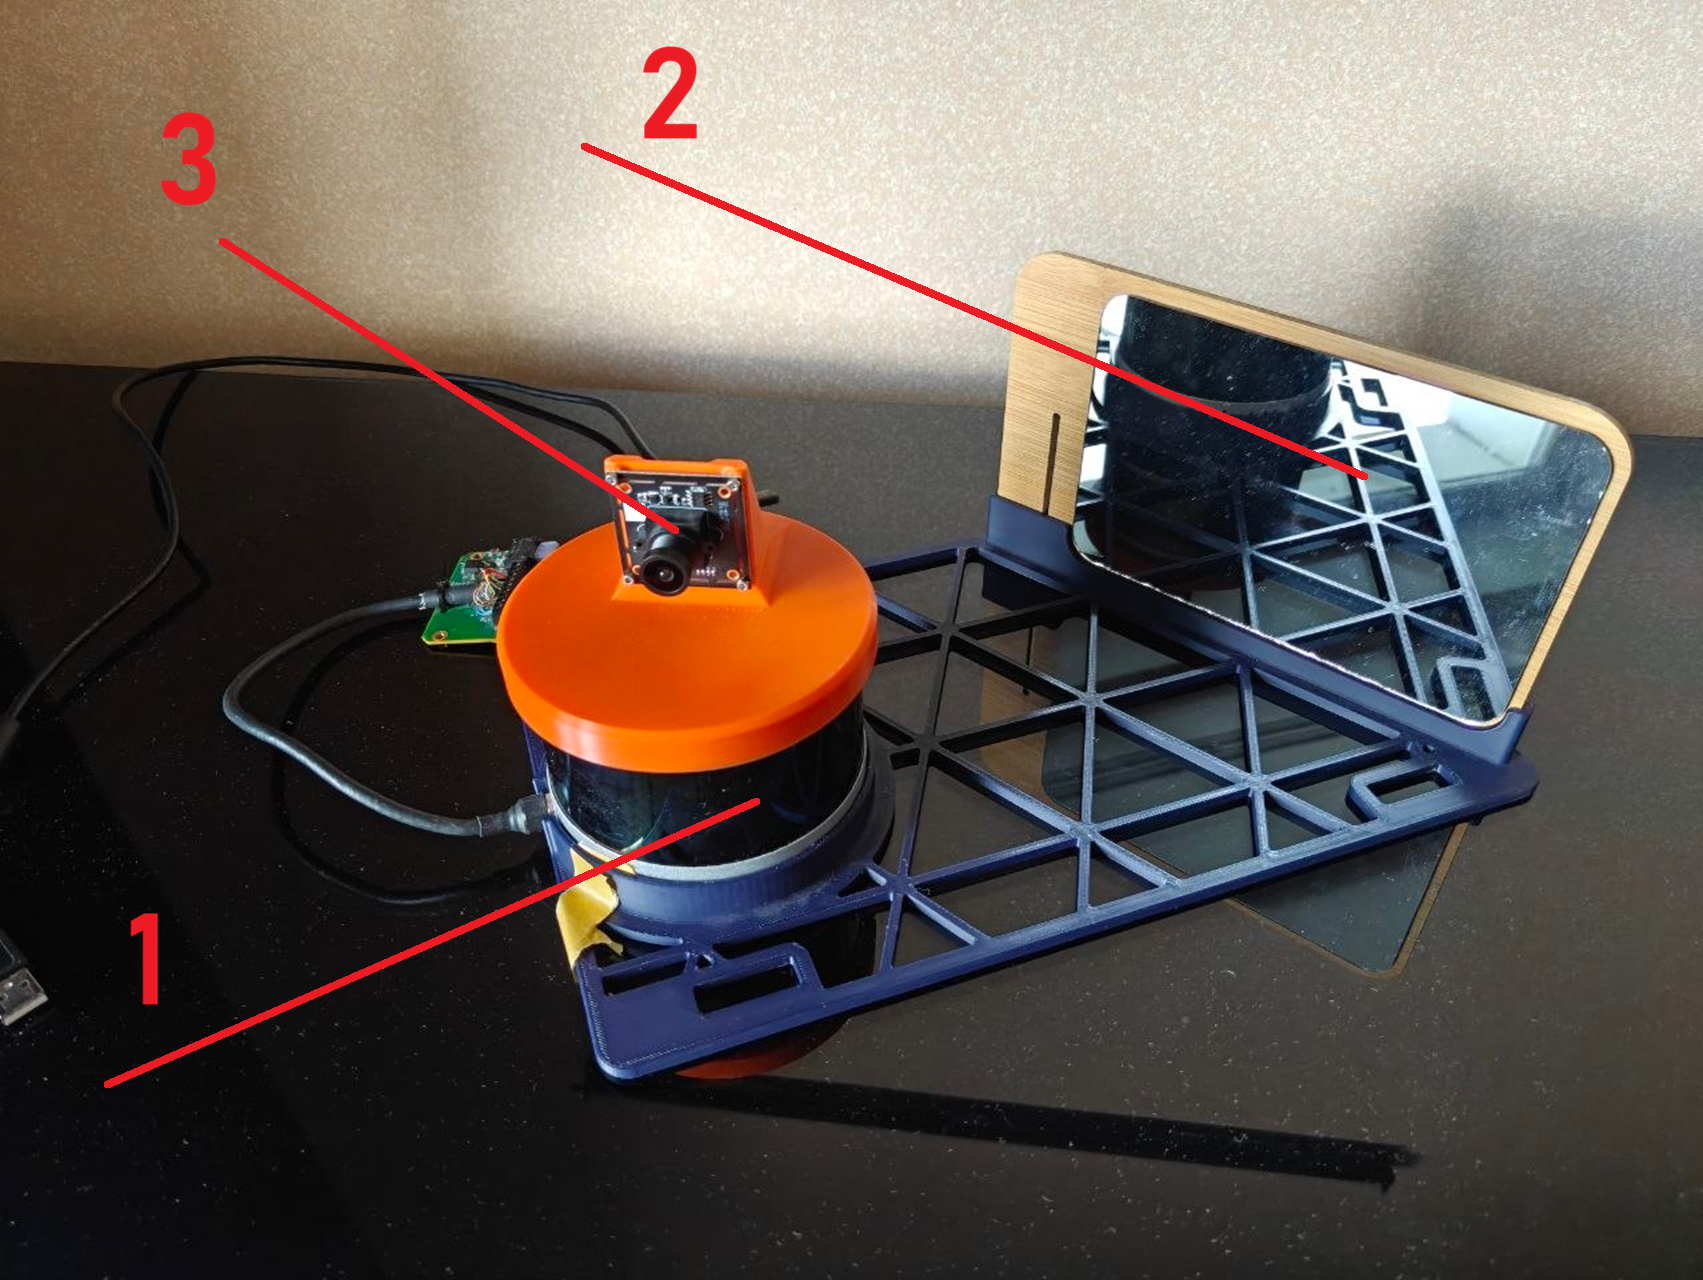
\includegraphics[width=\linewidth]{figures/setup.png}
  \end{minipage}
  \caption{Экспериментальная установка: 1 — LiDAR-сенсор; 2 — зеркало; 3 — модуль камеры.}
  \label{fig:setup}
\end{figure}

Основные параметры сенсоров, алгоритма ICP-калибровки зеркала и
конвейера цветовой регистрации сведены в таблицу~\ref{tab:params}.
Внутренние параметры камеры получены методом Жанга~\cite{Zhang2000Calibration}
по шахматной мишени; средняя ошибка репроекции на калибровочном наборе
составила $\sim 0{,}5$~пикс. Для оценки калибровки использована
последовательность \texttt{8\_flor\_misis\_2}, записанная в
формате MCAP на восьмом этаже НИТУ МИСИС в статичном коридорном
интерьере длительностью $78{,}35$~с: $1553$ облака точек \linebreak
($\sim 19{,}7$~Гц) и $2354$ кадра камеры ($\sim 29{,}9$~Гц); суммарно
$3907$ сообщений.

\begin{table}[t]
  \centering
  \caption{Параметры сенсоров и алгоритмов.}
  \label{tab:params}
  \resizebox{\linewidth}{!}{%
  \begin{tabular}{ll}
    \hline
    \textbf{Параметр} & \textbf{Значение} \\
    \hline
    \multicolumn{2}{l}{\textit{Лидар (Velodyne VLP-16)}} \\
    Число каналов & 16 \\
    Дальность, точность & до $100$~м; $\pm 3$~см~\cite{VLP16Manual} \\
    Частота публикации кадров & $\sim 19{,}7$~Гц \\
    Углы обзора, гор.\,/\,верт. & $360^{\circ}$ / $30^{\circ}$ \\
    Угловое разрешение, гор.\,/\,верт. & $0{,}1$--$0{,}4^{\circ}$ / $2^{\circ}$ \\
    \hline
    \multicolumn{2}{l}{\textit{Камера (Microdia USB)}} \\
    Разрешение & $640 \times 480$ \\
    Частота публикации кадров & $\sim 29{,}9$~Гц \\
    $(f_x, f_y; c_x, c_y)$ & $(488{,}62;\ 488{,}08;\ 319{,}10;\ 266{,}91)$ \\
    Дисторсия $(k_1, k_2, p_1, p_2, k_3)$ &
      $(-0{,}401;\ 0{,}156;\ 4{,}9{\cdot}10^{-4};$
      $\ 9{,}8{\cdot}10^{-5};\ 0)$ \\
    \hline
    \multicolumn{2}{l}{\textit{ICP-калибровка зеркала}} \\
    Воксельный фильтр (размер листа) & $0{,}1$ м \\
    ICP: макс. расстояние соответствия & $0{,}2$ м \\
    ICP: макс. число итераций & 30 \\
    Коэффициенты усиления $(g_x, g_y, g_\psi)$ & $(0;\; 0{,}5;\; 0{,}5)$ \\
    Параметры зеркала после калибровки &
      $(c_x, c_y, c_z, \psi, w)$ \\
      & $(0{,}2264;\; 0{,}0052;\; 0;\; 32{,}093^\circ;\; 0{,}18)$~м \\
    Порог обновления по норме поправки & $10^{-3}$ \\
    Порог останова по $E$ ($\varepsilon$) & $1{,}2$~м \\
    \hline
    \multicolumn{2}{l}{\textit{Цветовая регистрация}} \\
    Синхронизация облако--кадр (slop) & $0{,}1$ с \\
    Фильтр проекции $z_C$ & $> 0{,}1$ м \\
    Формат публикуемого RGB & PointCloud2 (\texttt{rgb} UINT32) \\
    \hline
  \end{tabular}%
  }
\end{table}

\subsection{Калибровка положения зеркала}

Калибровка выполнялась по следующему протоколу. Параметры зеркала
устанавливались в рабочую конфигурацию
$c = (0{,}2264;\; 0{,}0052;\; 0)$~м, $\psi = 32{,}093^{\circ}$
(получена ручной инициализацией $\psi_0 = 30^{\circ}$,
$c_{y,0} = 0$). Затем вводилось известное рассогласование по углу
$\psi$ и/или смещению $(c_x, c_y)$, после чего запускался контур
калибровки; фиксировались значение $E$~\eqref{eq:rmse} в момент
остановки контура и факт сходимости ICP.

На этапе ICP-калибровки ширина зеркала $w$ ещё не известна, поэтому
фрустум не настроен --- разбиение облака выполняется в предположении
бесконечной плоскости. Порог останова установлен
$\varepsilon = 1{,}2$~м.

Результаты семи экспериментов с различными комбинациями начальных
рассогласований приведены в таблице~\ref{tab:calib-series}.

\begin{table}[t]
  \centering
  \caption{Результаты серии запусков контура калибровки при различных
    начальных рассогласованиях (бесконечная плоскость,
    $\varepsilon = 1{,}2$~м); $E$ --- значение~\eqref{eq:rmse} в момент
    остановки контура.}
  \label{tab:calib-series}
  \resizebox{\linewidth}{!}{%
  \begin{tabular}{cccccc}
    \hline
    № & $\Delta\psi_0$, град. & $\Delta x_0$, мм &
      $\Delta y_0$, мм & $E$, м & Сходимость \\
    \hline
    1 & $ 0{,}0$ &    $0$ &    $0$ & $1{,}19$ & да \\
    2 & $-3{,}0$ &    $0$ &    $0$ & $1{,}10$ & да \\
    3 & $+3{,}0$ &    $0$ &    $0$ & $1{,}17$ & да \\
    4 & $ 0{,}0$ & $+10$ &    $0$ & $1{,}18$ & да \\
    5 & $ 0{,}0$ &    $0$ & $+10$ & $1{,}11$ & да \\
    6 & $+3{,}0$ & $+10$ & $+10$ & $1{,}15$ & да \\
    7 & $-5{,}0$ & $+20$ & $-20$ & $1{,}00$ & да \\
    \hline
  \end{tabular}%
  }
\end{table}

Во всех семи запусках ICP сошёлся, и контур остановился ниже порога
$\varepsilon = 1{,}2$~м независимо от начального рассогласования.
Значение порога подобрано под масштаб $E$ для данной сцены.
Поскольку остановка происходит на первом кадре с $E < \varepsilon$,
значения $E$ в таблице~\ref{tab:calib-series} лежат непосредственно
ниже порога и характеризуют кадр остановки, а не точность калибровки
(см. раздел~3); серия демонстрирует устойчивость сходимости контура к
начальным рассогласованиям вплоть до $\pm 5^{\circ}$ по углу и
$\pm 20$~мм по смещению. Итоговые параметры зеркала после калибровки
($\psi = 32{,}093^{\circ}$, $c_y = 5{,}2$~мм) приведены в
таблице~\ref{tab:params}. После сходимости
контура и фиксации $(c, \psi)$ выполняется ручная калибровка ширины
$w$ (п.~\ref{sec:icp-calib}), после чего фрустум настраивается и
разбиение облака уточняется.

Качественный результат калибровки --- совмещение отражённого облака с
прямым --- показан на рис.~\ref{fig:clouds}.

\begin{figure}[t]
  \centering
  \begin{minipage}{\linewidth}
    \centering
    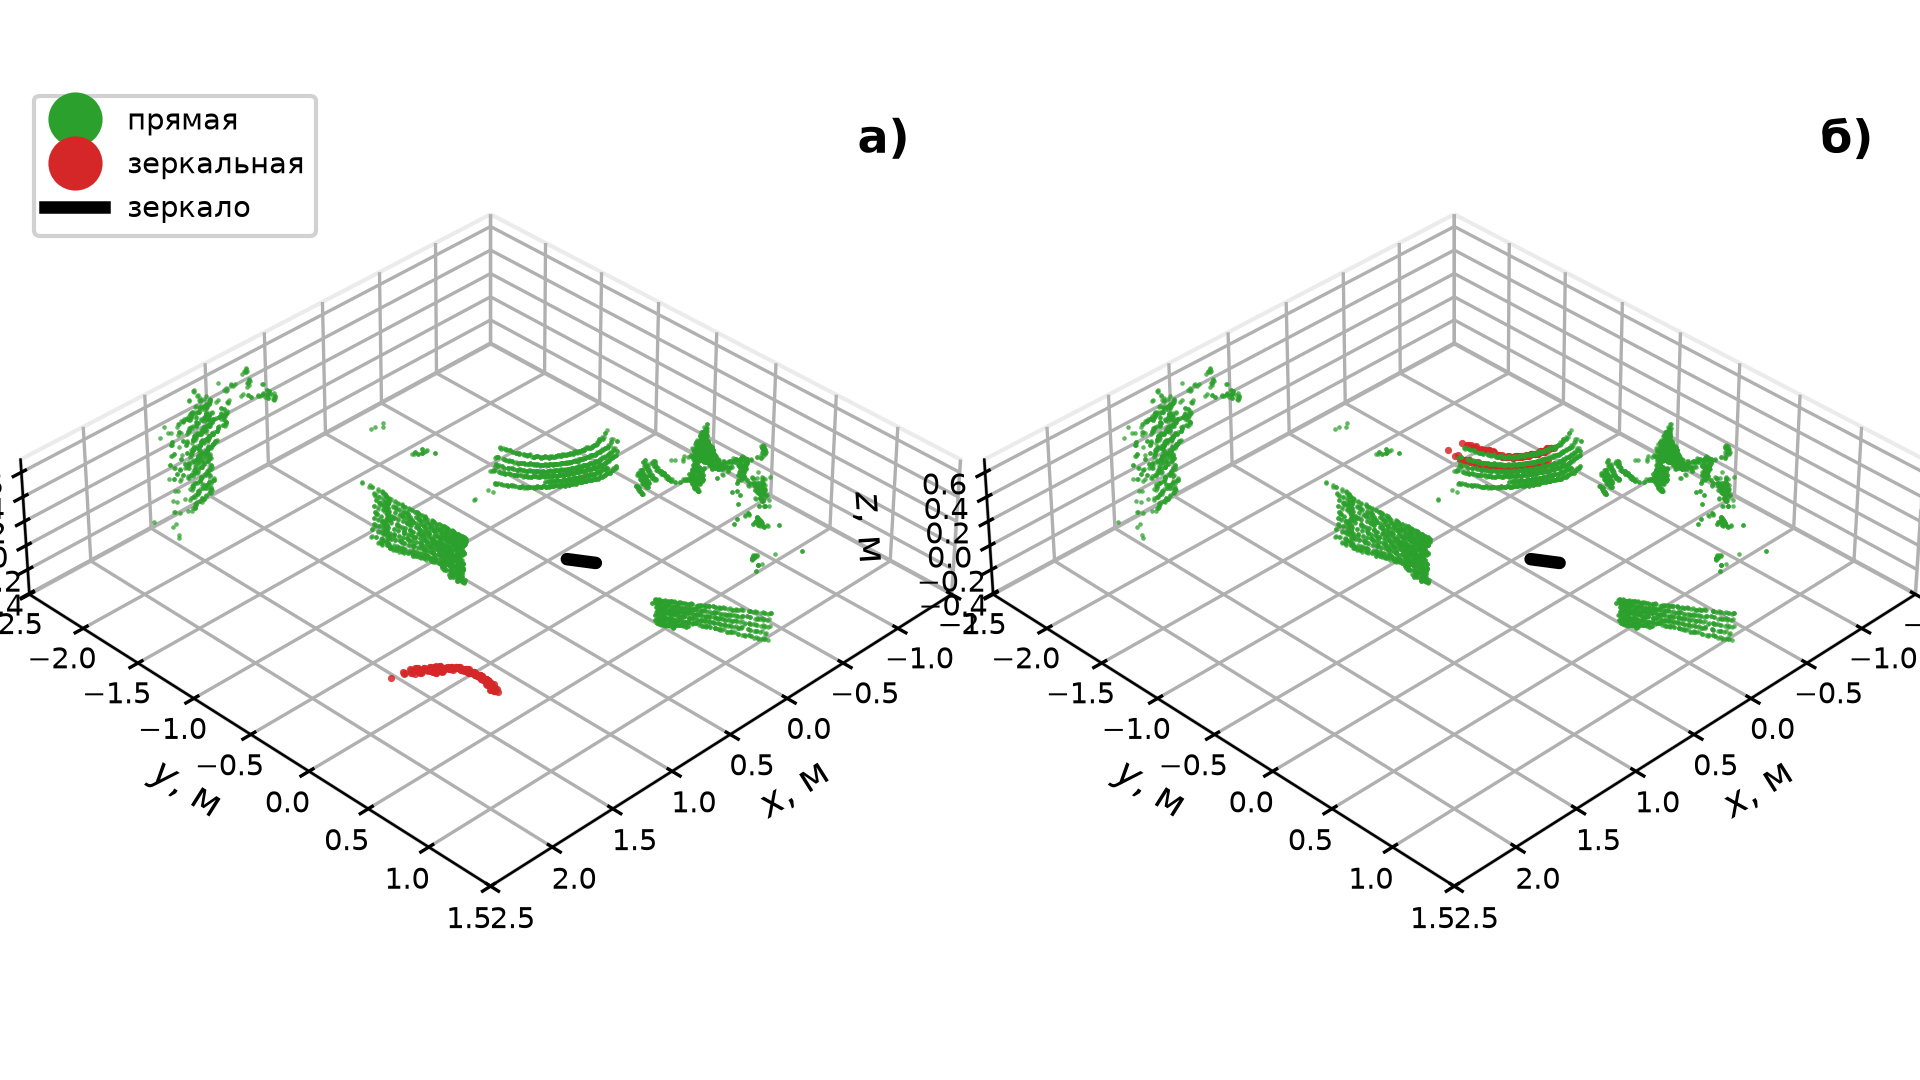
\includegraphics[width=\linewidth]{figures/clouds_final.png}
  \end{minipage}
  \caption{Облака точек: (а) исходное облако с разделением на прямую
    (зелёным) и зеркальную (красным) части, чёрным отрезком показано
    зеркало; (б) объединённое облако после калибровки (зеркальная часть
    отражена по откалиброванным параметрам). Показан фрагмент сцены
    радиусом $\sim 2$~м вокруг сенсора.}
  \label{fig:clouds}
\end{figure}

\subsection{Цветовая регистрация}

Внешняя калибровка камера--лидар выполнена интерактивно на записи
статичной сцены с использованием разработанного графического инструмента
(\texttt{colorize\_live.py}), позволяющего в реальном времени
наблюдать проекцию облака точек на кадр камеры и подстраивать четыре
параметра $(t_x, t_y, t_z, \varphi)$ ползунками с задержкой обновления
$80$~мс. Полученные значения:
$t_{lc} = (-0{,}066;\; -0{,}010;\; -0{,}188)$~м, $\varphi =
121{,}25^{\circ}$ (матрица поворота --- по формуле~\eqref{eq:rlc}).
Пример покрашенного объединённого облака приведён на
рис.~\ref{fig:colored}: видно, что отражённый (зеркальный) канал
получает цвета, согласованные с прямым каналом.

\begin{figure}[t]
  \centering
  \begin{subfigure}[b]{0.48\linewidth}
    \centering
    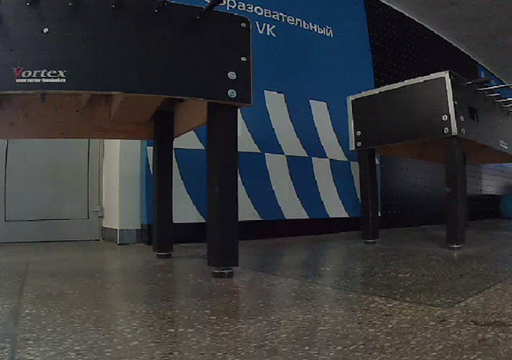
\includegraphics[width=\linewidth]{figures/image_from_camera.png}
    \caption{кадр камеры}
    \label{fig:colored:camera}
  \end{subfigure}\hfill
  \begin{subfigure}[b]{0.48\linewidth}
    \centering
    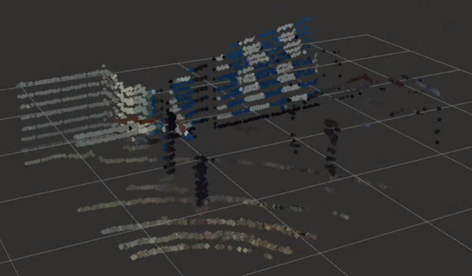
\includegraphics[width=\linewidth]{figures/colored_cloud.png}
    \caption{покрашенное объединённое облако}
    \label{fig:colored:cloud}
  \end{subfigure}
  \caption{Цветовая регистрация объединённого облака точек:
    (а) кадр камеры; (б) покрашенное объединённое облако
    (прямой и зеркальный каналы).}
  \label{fig:colored}
\end{figure}

Количественные характеристики цветовой регистрации оценивались на
последовательности \texttt{8\_flor\_misis\_2} (табл.~\ref{tab:params}).
Прямой канал VLP-16 с горизонтальным углом обзора $360^{\circ}$
формирует существенно более широкое покрытие, чем поле зрения камеры;
последнее оценивается сверху величиной $\mathrm{FoV}_x \approx 2\arctan(
W/(2 f_x)) \approx 66^{\circ}$ по горизонтали и
$\mathrm{FoV}_y \approx 52^{\circ}$ по вертикали. Соответственно
доля точек прямого канала, попадающих в кадр камеры, для типичного
скана $t = 30$~с записи составила
$N_{\text{кадр}}/N \approx 0{,}18$; ещё $\sim 0{,}06$ точек добавляет
зеркальный канал (лидар видит через зеркало часть той же сцены), что
даёт итоговую долю $\sim 0{,}24$. Прирост числа окрашенных точек за
счёт зеркального канала на этом кадре составил
$+33\%$ по отношению к прямому каналу.
Дополнительно на объединённом облаке
$P_{\text{total}} = P_n \cup P_m^{*}$, накопленном за всю запись
($\sim 2{,}3 \cdot 10^{7}$ точек после препроцессинга), применение
воксельной метрики плотности из п.~\ref{sec:icp-calib} даёт прирост
среднего числа точек на воксель $D$ во всём исследованном диапазоне
разрешений и наиболее выраженный прирост занятости $\Delta C$ при
шаге сетки $V = 0{,}1$--$0{,}25$~м, что согласуется с ранее полученными
данными натурного эксперимента~\cite{VisFed26}.

Для верификации интерактивно найденной $T_{lc}$ дополнительно применён
метод автоматической targetless-калибровки
\cite{Koide2023GeneralCalib} на той же последовательности
\texttt{8\_flor\_misis\_2}: препроцессированное облако из
$2{,}3 \cdot 10^{7}$ точек и синхронизированные кадры камеры,
интринзики из табл.~\ref{tab:params}. Оптимизация с интерактивно
подобранной $T_{lc}$ в качестве начального приближения сошлась за
$\sim 15$~мин; уменьшение целевой функции NID (нормализованной
информационной дистанции)~\cite{Koide2023GeneralCalib}
подтвердило корректность начальной оценки, при этом визуальное
качество проекции облака на кадр в интерактивно найденной
конфигурации оказалось выше, чем в автоматически уточнённой. Это
характерное поведение метода NID в интерьерных сценах с ограниченным
разнообразием текстур --- к обсуждению возвращаемся в разделе~5.

% ============================================================
\section{Обсуждение результатов}

Проведённые эксперименты показывают, что обе поставленные задачи
решаются на реальном оборудовании в автоматическом или
полуавтоматическом режиме. Калибровка положения зеркала выполняется по
данным самого лидара, без калибровочных мишеней, и сходится в темпе
поступления кадров; в отличие от подхода работы
\cite{Kibii2022MirrorCalibration}, не требуется отдельная процедура с
известной геометрией сцены. По сравнению с предыдущей работой авторов
\cite{VisFed26}, где метод зеркального усиления
исследовался преимущественно в симуляции, в настоящей работе замкнутая
система --- разделение каналов, калибровка зеркала, цветовая
регистрация --- реализована и проверена на физической установке.

Вместе с тем подход имеет ряд ограничений, определяющих направления
его развития.

Во-первых, модель зеркала предполагает вертикальную установку: нормаль
параметризуется единственным углом $\psi$~\eqref{eq:normal}. Наклон
зеркала относительно вертикали в текущей модели не учитывается и
приводит к систематической ошибке отражения; переход к полной
трёхмерной параметризации нормали ($\psi$, $\theta$) является
естественным обобщением.

Во-вторых, наблюдаемость параметров не полна: отражение~\eqref{eq:reflect}
зависит от положения плоскости только через проекцию центра на нормаль
$c^{\top} n$, поэтому контур восстанавливает лишь одну поступательную
степень свободы зеркала; в используемой конфигурации калибруется $c_y$,
а $c_x$ фиксируется ручной инициализацией ($g_x = 0$). Кроме того,
контур требует грубой начальной оценки положения зеркала: при больших
начальных рассогласованиях ICP сходится к ложному локальному минимуму.
Автоматизация инициализации --- отдельная задача.

В-третьих, метрика $E$~\eqref{eq:rmse} вычисляется по всем
соответствиям без отсечки и потому определяется главным образом
геометрией сцены: порог останова $\varepsilon$ не ограничивает
напрямую ошибку калибровки, а качество совмещения контролируется
визуально по объединённому облаку. Кроме того, точность калибровки
ограничена снизу характеристиками сенсора: заявленная точность
дальнометрии VLP-16 составляет $\pm 3$~см~\cite{VLP16Manual}, что
определяет физический предел согласования облаков независимо от
порога остановки контура.

В-четвёртых, цветовая регистрация не учитывает взаимные окклюзии:
точки, которым в кадре камеры соответствует фоновый объект, получают
некорректный цвет. Строгое решение требует z-буферизации проекции или
построения поверхности сцены. Кроме того, интерактивная калибровка
$T_{lc}$ выполняется вручную и зависит от оператора; перспективна её
замена автоматической targetless-калибровкой камера--лидар. Опыт
применения такого метода (реализация~\cite{Koide2023GeneralCalib},
основанная на минимизации нормализованной информационной дистанции
между интенсивностью проекции лидара и яркостью изображения) на
записи \texttt{8\_flor\_misis\_2} показал, что в интерьерной сцене с
малым разнообразием текстур (однородные стены коридора) целевая
функция NID имеет слабо выраженный минимум и алгоритм чувствителен к
качеству начального приближения; в наших условиях интерактивно
найденная $T_{lc}$ давала лучший визуальный результат, чем
автоматически уточнённая. Для сцен с богатыми текстурами (уличные
кадры, кампусы) targetless-калибровка предположительно останется
более точной; выбор метода в общем случае определяется характером
сцены.

Наконец, все эксперименты проведены на статичных сценах; перенос на
динамические сцены потребует временн\'{о}й синхронизации сенсоров и
учёта движения объектов. Кроме того, серия калибровок выполнена на
одной интерьерной сцене и характеризует устойчивость контура к
начальному рассогласованию; проверка на других сценах и положениях
зеркала --- направление дальнейшей работы.

% ============================================================
\section{Выводы и заключение}

В работе рассмотрены две взаимосвязанные задачи, возникающие при
практическом построении зеркально-усиленной лидарной системы, и
предложены их решения.

Во-первых, предложен метод автоматической калибровки положения плоского
зеркала относительно лидара: облако точек разделяется на прямую и
отражённую части по модели зеркального канала, а параметры зеркала
итеративно уточняются алгоритмом ICP в контуре обратной связи
реального времени, без калибровочных мишеней и с численным контролем
сходимости по среднеквадратичной ошибке совмещения.

Во-вторых, построен конвейер цветовой регистрации объединённого
(прямого и отражённого) облака точек по изображению камеры с
интерактивной калибровкой четырёх внешних параметров камера--лидар.

В-третьих, оба метода реализованы в виде пакетов ROS~2
(\texttt{icp\_registration} на C++/PCL и \texttt{colorize\_live\_pkg}
на Python/OpenCV) и апробированы на реальной установке
(Velodyne VLP-16, плоское зеркало, USB-камера $640\times 480$) на
записи длительностью $78$~с из статичного коридорного интерьера. На
серии из семи запусков из различных начальных рассогласований
ICP-контур сходился во всех случаях; итоговые параметры зеркала
составили $\psi = 32{,}1^{\circ}$, $c_y = 5{,}2$~мм. Цветовая
регистрация объединённого облака дала $\sim 24\%$ окрашенных точек с
приростом $\sim 33\%$ за счёт зеркального канала. Предложена
воксельная метрика прироста плотности облака за счёт зеркального
канала.

Направления дальнейшей работы: автоматическая инициализация контура
калибровки; переход к полной трёхмерной параметризации зеркала
(наклонные зеркала); учёт окклюзий при цветовой регистрации и
автоматическая targetless-калибровка камера--лидар; эксперименты на
динамических сценах; использование зеркально-усиленных цветных облаков
в сквозных задачах, в частности в сегментации облаков точек.

% ============================================================
\section*{Благодарности}

Исследование выполнено при поддержке кафедры инженерной кибернетики НИТУ МИСИС.

% ============================================================
% Список литературы (перенесён из references.bib исходной статьи)
\begin{thebibliography}{99}

\bibitem{khoshelham2018benchmark} Kumar U.~R., Coudron I., Puttemans S., Vandewalle P. Quality Assessment for 3D Reconstruction of Building Interiors. \textit{Journal of Imaging Science and Technology}, vol.~62, no.~1, pp.~010402-1--010402-10, 2018.

\bibitem{VisFed26} Вишневский~М.~Р., Фёдоров~И.~Ю. Повышение пространственного разрешения механических LiDAR-систем с использованием виртуального зеркального канала и автоматической калибровки. \textit{Труды ИСП РАН}, т.~38, вып.~3(3), с.~101--114, 2026.

\bibitem{Matsubara2020MirrorLiDAR} Matsubara K., Nagatani K., Hirata Y. Improvement in Measurement Area of 3D LiDAR for a Mobile Robot Using a Mirror Mounted on a Manipulator. \textit{2020 IEEE/RSJ International Conference on Intelligent Robots and Systems (IROS)}, pp.~9523--9530, 2020.

\bibitem{Pogacnik2022MultiperspectiveLiDAR} Pogacnik M., Munih M. Towards a Multi-Perspective Time of Flight Laser Ranging Device Based on Mirrors and Prisms. \textit{Applied Sciences}, vol.~12, no.~14, p.~7121, 2022.

\bibitem{Kibii2022MirrorCalibration} Kibii J.~E., Dreher A., Wormser P.~L., Gimpel H. Design and Calibration of Plane Mirror Setups for Mobile Robots with a 2D-Lidar. \textit{Sensors}, vol.~22, no.~20, p.~7830, 2022.

\bibitem{fastlio2} Xu W., Cai Y., He D., Lin J., Zhang F. FAST-LIO2: Fast Direct LiDAR-Inertial Odometry. \textit{IEEE Transactions on Robotics}, vol.~38, no.~4, pp.~2053--2073, 2022.

\bibitem{r3live} Lin J., Zhang F. R3LIVE: A Robust, Real-time, RGB-colored, LiDAR-Inertial-Visual tightly-coupled state Estimation and mapping package. arXiv:2109.07982, 2021.

\bibitem{Besl1992ICP} Besl P.~J., McKay N.~D. A Method for Registration of 3-D Shapes. \textit{IEEE Transactions on Pattern Analysis and Machine Intelligence}, vol.~14, no.~2, pp.~239--256, 1992.

\bibitem{Rusu2011PCL} Rusu R.~B., Cousins S. 3D is here: Point Cloud Library (PCL). \textit{2011 IEEE International Conference on Robotics and Automation (ICRA)}, pp.~1--4, 2011.

\bibitem{Zhang2000Calibration} Zhang Z. A Flexible New Technique for Camera Calibration. \textit{IEEE Transactions on Pattern Analysis and Machine Intelligence}, vol.~22, no.~11, pp.~1330--1334, 2000.

\bibitem{VLP16Manual} Velodyne LiDAR, Inc. VLP-16 User Manual, 2019. URL: \url{https://velodynelidar.com/wp-content/uploads/2019/12/63-9243-Rev-E-VLP-16-User-Manual.pdf} (дата обращения: 31.07.2026).

\bibitem{Koide2023GeneralCalib} Koide K., Oishi S., Yokozuka M., Banno A. General, Single-shot, Target-less, and Automatic LiDAR-Camera Extrinsic Calibration Toolbox. arXiv:2302.05094, 2023.

\end{thebibliography}

\end{document}
